% !TEX root = ../../thesis.tex

\section{Intertext UIDL} \label{intertextUIDL}

The Intertext UIDL (IUIDL) is an XML-based markup language that can be used to describe user interfaces. It features a layout system and UI components that could be used as building blocks to put together a user interface. IUIDL is meant to be served from a generic backend, assembled on the backend based on the application logic. It is designed to be unopinionated, as it does not restrict how you assemble it or serve it, or where you serve it from. For instance, below is an example To-do list UI served in IUIDL from a Node.js server that uses Express.js framework, as shown in Figure \ref{fig:todos_js}. Once hit, the endpoint \texttt{/todo} passes the To-do item data to a template file which uses Handlebar as a template engine, and it renders the UI in IUIDL format. The output XML is served from the endpoint.

\begin{figure}
\begin{minipage}{\linewidth}
\begin{lstlisting}[language=javascript]
router.get('/todo', function(req, res, next) {

  const todos = [
    {
      title: 'Buy milk',
      done: false,
    },
    {
      title: 'Call mom',
      done: false,
    },
    {
      title: 'Prepare for presentation',
      done: true,
    },
  ];

  res.render('todo', {
    itemsToDo: todos.filter(item => !item.done),
    itemsDone: todos.filter(item => item.done),
  });
});
\end{lstlisting}
\end{minipage}
\caption{A simple Express endpoint that serves the render output of the Handlebars template shown in Figure \ref{fig:todos_template}}%
\label{fig:todos_js}%
\end{figure}

\begin{figure}
\begin{minipage}{\linewidth}
\begin{lstlisting}[language=xml]
<h3>To do ({{ itemsToDo.length }})</h3>

{{#each itemsToDo}}
  <block intent="default" flexDirection="row" alignItems="center" paddingLeft="4">
    <text flexGrow="1">{{this.title}}</text>
    <button intent="error">Remove</button>
    <button intent="success" marginLeft="2">Done</button>
  </block>
{{/each}}


<h3>Done ({{ itemsDone.length }})</h3>

{{#each itemsDone}}
  <block intent="default" flexDirection="row" alignItems="center" paddingLeft="4">
    <text flexGrow="1">{{this.title}}</text>
    <button intent="error">Remove</button>
  </block>
{{/each}}
\end{lstlisting}
\end{minipage}
\caption{Handlebars template that renders To-do items in IUIDL format}%
\label{fig:todos_template}%
\end{figure}

\begin{figure}
  \centering
  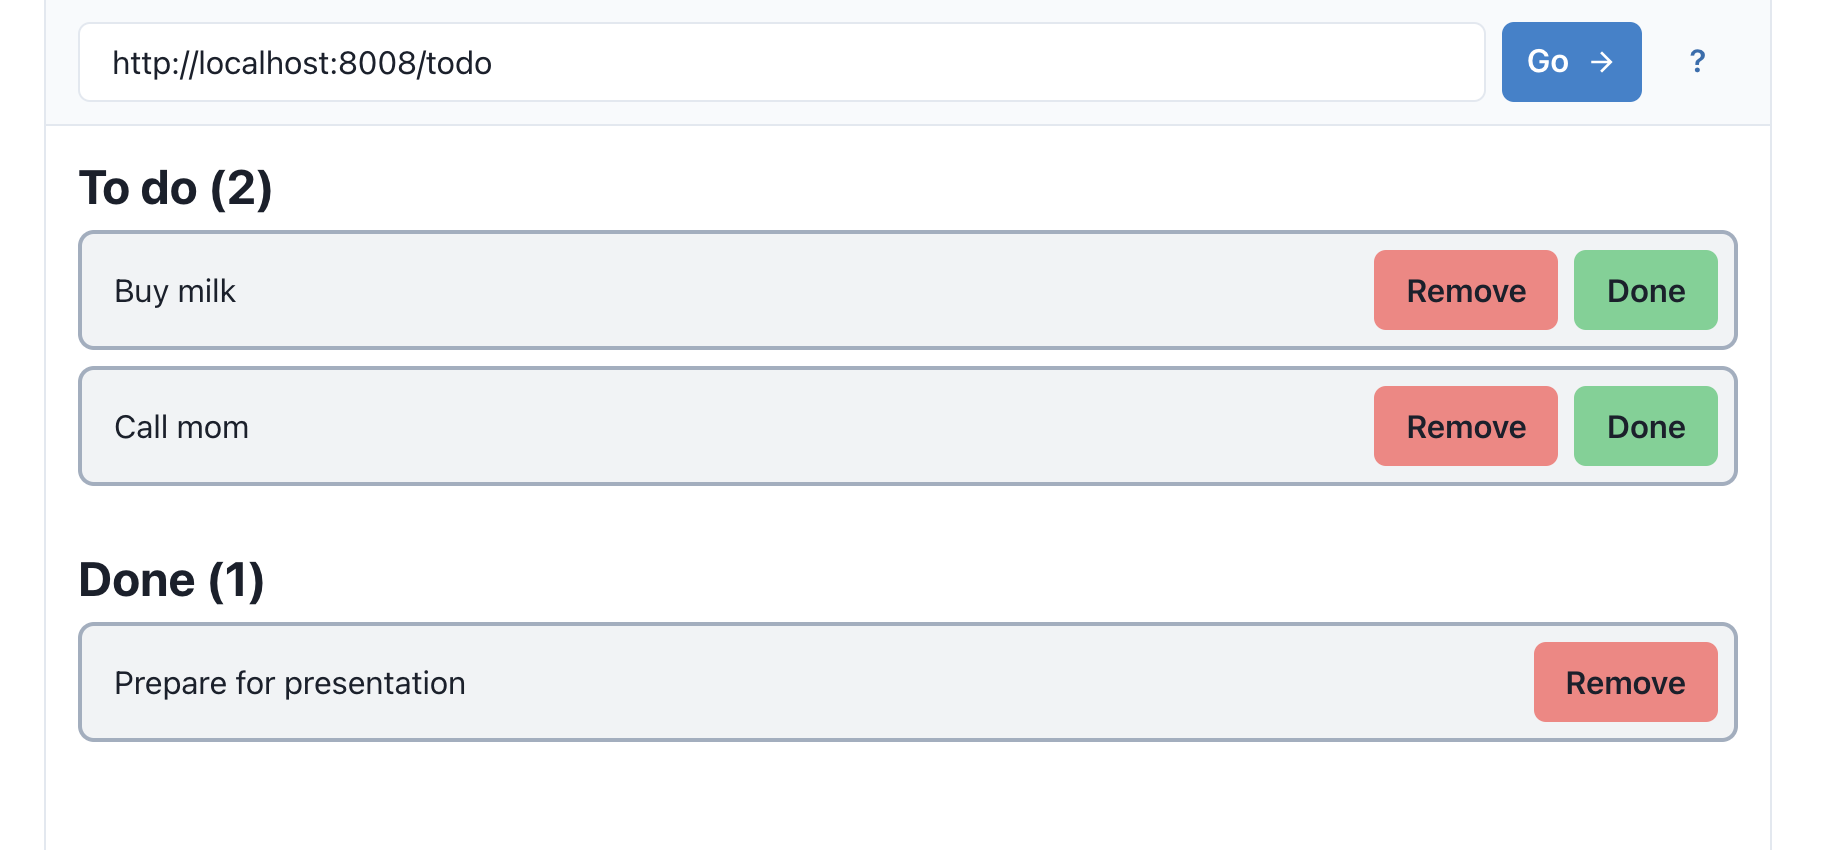
\includegraphics[width=13cm]{thesis/paper/images/todos.png}
  \caption{IUIDL served from the endpoint in Figure \ref{fig:todos_js} rendered on the Intertext web client}%
  \label{fig:todos_output}%
\end{figure}

\subsection{Styling}

IUIDL is agnostic of the styling. There are several \textit{intent}'s that components can accept, which renders the component most appropriately based on its use case. For instance, the Remove buttons in Figure \ref{fig:todos_output} as can be seen as red, and Done buttons green. That is because the \textit{error} intent was given to the Remove button and \textit{success} intent was given to the Done button. However, in this configuration, there is no way to specify how the components look like in particular. The main idea is customisability. Intertext provides themes that users can choose from, and for each theme UI components look and feel differently. Currently, only light and dark themes are available for the web version of Intertext (the dark version of the To-do list UI can be seen in Figure \ref{fig:todos_output_dark}), but as mentioned in the \nameref{futureWork} section, more themes will be made available. Moreover, users will also be able to create custom themes that exactly match their liking.

\begin{figure}
  \centering
  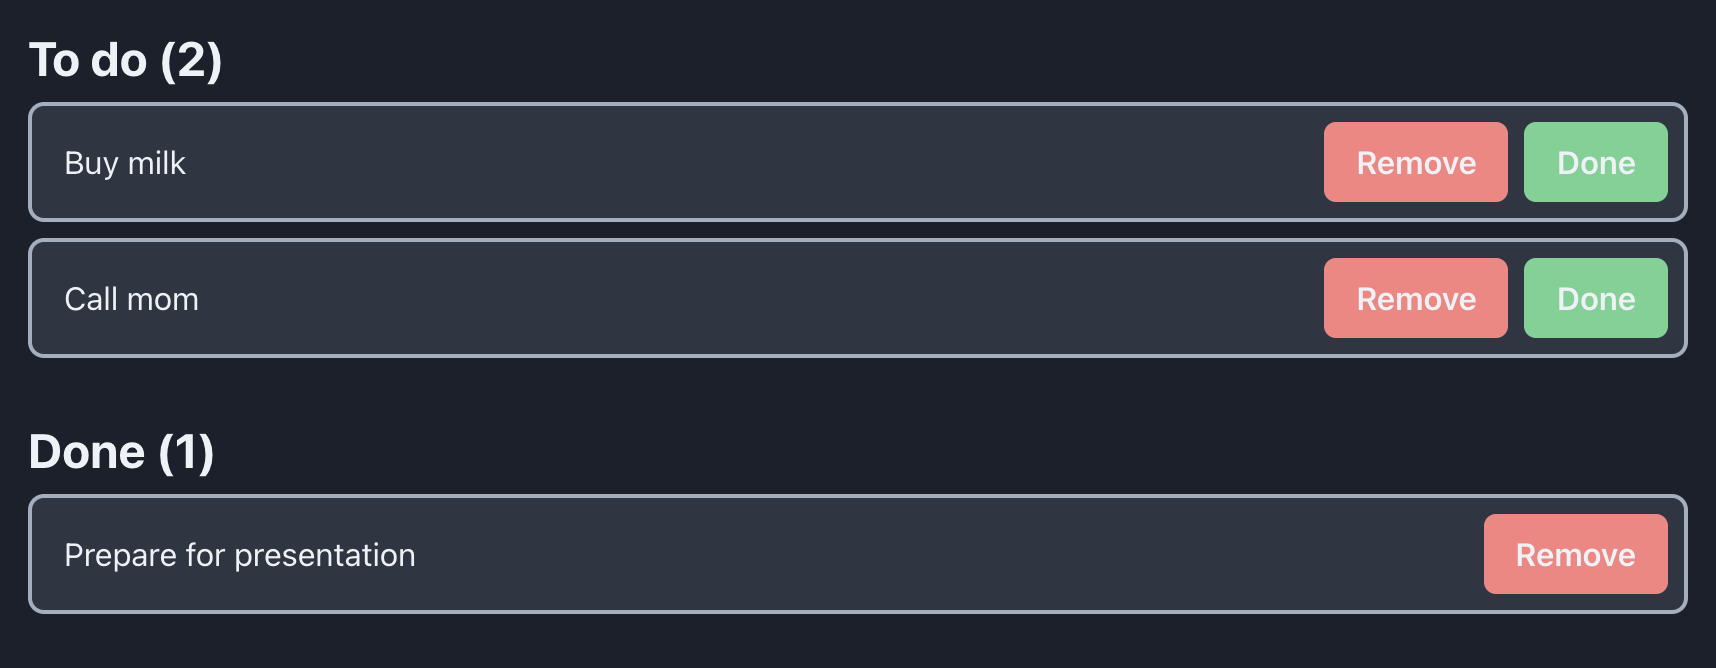
\includegraphics[width=13cm]{thesis/paper/images/todos_dark.png}
  \caption{Dark version of the To-do list UI from Figure \ref{fig:todos_output} rendered on Intertext web client}%
  \label{fig:todos_output_dark}%
\end{figure}

\subsection{Syntax}

As explained in detail in the \nameref{implementation} section, IUIDL gets converted from XML syntax to JSON syntax. However, the conversion to JSON is only an implementation detail that takes place during the rendering phase, and developers do not need to be aware of. XML was chosen at the cost of creating an additional transpilation layer, to achieve optimum developer friendliness. 

When it comes to building UIs, XML and XML-like languages are very common. The main benefit of such languages is that they are easy to read and write, while at the same time they are easy to parse and process as data. IUIDL is meant to be served from a backend, but developers still need to write IUIDL code by hand on the server side. JSON is far from being practical to write in large by hand. The difference could be observed in Figure \ref{fig:syntax_json} and Figure \ref{fig:syntax_xml}, the IUIDL code for a custom 404 page could be seen in both XML and JSON syntax.

\begin{figure}
\begin{minipage}{\linewidth}
\begin{lstlisting}[language=xml]
<block intent="error">
  <h3 intent="error">Not Found</h3>
  <collapse>
    <collapse.handle>
      <text intent="error">
        Show Details
      </text>
    </collapse.handle>
    <p intent="error">... stack trace here ...</p>
  </collapse>
</block>
\end{lstlisting}
\end{minipage}
\caption{The XML representation of the 404 page}%
\label{fig:syntax_xml}%
\end{figure}

\begin{figure}
\begin{minipage}{\linewidth}
\begin{lstlisting}[language=json]
[
    {
        "block": [
            {
                "h3": "Not Found",
                "intent": "error"
            },
            {
                "collapse": [
                    {
                        "p": "... stack trace here ...",
                        "intent": "error"
                    }
                ],
                "handle": [
                    {
                        "text": "\n        Show Details\n      ",
                        "intent": "error"
                    }
                ]
            }
        ],
        "intent": "error"
    }
]
\end{lstlisting}
\end{minipage}
\caption{The JSON representation of the 404 page}%
\label{fig:syntax_json}%
\end{figure}


One issue that raised from the XML syntax was the inability to assign complex children to attributes of a specific tag. As it can be seem from the JSON representation of the 404 page in Figure \ref{fig:syntax_json}, the component \texttt{collapse} requires two sets of children: one for its direct children (specified as \texttt{collapse}), and one for the children to be rendered in its handle (specified as \texttt{handle}). Both \texttt{collapse} and \texttt{handle} properties take other UI components as their children. However, the XML syntax only allows attribute values of a tag to be of type string. In order to solve this problem, we extended XML to create a special syntax to handle such cases. We introduced a special tag name convention: when an XML tree is placed as the children of a component with the tag name being the parent components name concatenated with an attribute name joined together with a dot ("."), it gets interpreted as an attribute of the parent, with its value being the children of that XML tree (Figure \ref{fig:complex_attributes}).

\begin{figure}
\begin{minipage}{\linewidth}
\begin{lstlisting}[language=xml]
<parent>
  <parent.complex>
    <text>
      This is under 'complex' attribute of parent
    </text>
  </parent.complex>
  <text>
    This is the real children of parent
  </text>
</parent>
\end{lstlisting}
\end{minipage}
\caption{Complex attributes}%
\label{fig:complex_attributes}%
\end{figure}


\subsection{Terminology}

A last thing to mention in this section is the terminology used in IUIDL. The IUIDL syntax is shared between multiple devices and environments, which includes desktop interfaces as well as touch interfaces, non-graphical user interfaces and more. As mentioned in the \nameref{futureWork} section, as more Intertext clients gets released, the variety will further increase. This brings up a problem with the terminology. For instance, the \texttt{click} that normally would make sense for a desktop environment does not make sense for touch interfaces, as the interaction for a touch screen interface would be \texttt{touch} or \texttt{tap}. In the case of a command line, the primary interaction is focusing on an item and hitting the "enter" key. 

Our immediate reaction to solve this problem was to create custom jargon that is agnostic of device/interaction type, just like IUIDL is by nature, and find terms for every component/interaction that applies globally. For instance, instead of "button" we used \texttt{callToAction}, and instead of \texttt{onClick} we used \texttt{onPrimaryInteraction}. However we later abandoned this approach for the sake of developer friendliness. As we custom-named components and their respective actions, we realised that their names were getting very unusual and non-familiar, to a point where it was very difficult to even recognise them. Should we have chosen the global naming convention, we would have introduced a steep learning curve; developers would have needed to get familiar with a long list of terms that they have never heard of before, and they would strictly need to follow the documentation while building Intertext applications.

Instead, we decided to adopt the terminology for desktop/web environments. The rationale behind this decision was that these environments have been around for a very long time, that the terms used to build desktop applications and web applications has a strong recognition among many developers. Also, terms used for desktop environments were mostly generic enough that it was easy to represent on other environments. For instance, a \texttt{button} is a component to be interacted with that performs an action, and \texttt{click} is the method of primary interaction with that component. We can easily take this as a given to replicate it on any environment and create an optimised version taking the limitations of the host platforms in mind.